\documentclass[11pt]{article}

\usepackage[margin=1.15in]{geometry}
\usepackage{amsmath,amssymb}
\usepackage{booktabs}
\usepackage{graphicx}
\usepackage{caption}
\usepackage{microtype}
\usepackage[hidelinks]{hyperref}
\usepackage{enumitem}
\usepackage[numbers]{natbib}

\captionsetup{font=small, labelfont=bf, skip=8pt}
\setlist{itemsep=2pt, topsep=4pt}
\newcommand{\code}[1]{\texttt{\small #1}}

\title{\bfseries What Constrained Decoding Buys at High Item Counts:\\[2pt]
Validity, Not Recall}

\author{Raunak Sood\\
\normalsize University of Southern California\\
\normalsize \texttt{raunakso@usc.edu}}

\date{September 2026}

\begin{document}
\maketitle

\begin{abstract}
\noindent
Schema-constrained decoding is widely believed to cost accuracy, because forcing
output through a grammar masks tokens the model would otherwise emit. We measure
that cost along an axis it has not been measured on: the number of items the
model must produce. Holding input length constant by construction, we build
documents containing exactly $k$ verbatim-validated sentences, each naming one
entity, and vary $k$ from 1 to 16, with 25 documents per level on one model.
Under a pre-registered rejection rule (a recall drop of at least 0.15 from
$k \le 3$ to $k \ge 16$ and $p < 0.05$), neither decoding regime rejects the
null: unconstrained recall falls 0.131 (Spearman $-0.255$, $p = 0.027$) and
schema-constrained recall does not fall ($-0.114$, i.e.\ it rises; $p = 0.73$).
An earlier version of this paper reported a 0.214 drop and a rejection for the
unconstrained arm; six of its 75 responses had been scored as zero because the
tolerant parser rejected valid-looking JSON containing unescaped quotation marks
copied from the filings, and a repair step that recovers them is now part of the
scorer. Paired on identical documents, the gap between arms moves $-0.061$ per
doubling of $k$ ($p = 0.020$), but it is carried by $k = 1$, where the
constrained arm emits an empty list on 13 of 25 documents; without those
documents the interaction vanishes ($p = 0.17$). What does survive with an
artifact is validity: the share of responses that are valid JSON as emitted
falls with $k$ without a grammar (25/25, 23/25, 21/25) and is 75/75 under one.
The study's validity gate, recall of 0.80 at $k = 1$, was never met, so absolute
recall levels are not interpretable. We also show that item count, item density
and document length cannot be held fixed simultaneously, which determines
whether any measurement on this axis is an upper or a lower bound.
\end{abstract}

\section{Introduction}

Ask a language model for a list and it will sometimes give you a shorter one than
the document supports. Whether that tendency worsens as the list grows is an
empirical question with a measurable answer, and it has not been measured in the
setting where it matters most for production systems: structured extraction under
a schema.

Two literatures bracket the question without answering it. Long-context work
measures how retrieval degrades with input length and with the position of the
evidence~\citep{lostinmiddle,ruler,contextrot}, and multi-evidence variants
report that retrieval falls as the number of inserted facts
rises~\citep{multineedle,countingstars}. Long-list extraction is recognised as
hard enough to need retrieval augmentation and a pruning
stage~\citep{recallthemall}, and extraction benchmarks report performance
falling as schemas widen~\citep{extractbench}. Structured-output work measures
the cost of constrained decoding. The grammar masks tokens the model would
otherwise emit~\citep{outlines}; reported accuracy losses of several points on
reasoning tasks~\citep{letmespeak} are contested as artefacts of prompt
mismatch~\citep{saywhatyoumean} or of vocabulary
misalignment~\citep{domino}; grammar constraints help on structured NLP tasks
without finetuning~\citep{gcd2023}; and a benchmark over ten thousand schemas
measures validity, coverage and efficiency~\citep{jsonschemabench}. Closer to the present axis, \citet{sametask} show that reasoning
degrades as the same task is padded with more tokens, LongGenBench~\citep{longgenbench}
measures how long structured \emph{outputs} degrade with their required length,
and NoLiMa~\citep{nolima} separates retrieval from lexical matching in long
contexts. None of these varies the number of items to emit while holding input
length fixed, and none compares decoding regimes on that axis.

The distinction matters because the two candidate explanations make opposite
predictions. If degradation is a property of the model's attention over a long
list of targets, a grammar should not help. If it is a property of the model
choosing when to stop, a decoding regime that changes the stopping point should
help. At this scale the data do not decide between them: once a parser defect
is repaired (Section~\ref{sec:results}), neither arm meets the pre-registered
rejection rule, and the measurable difference the grammar makes is to output
validity rather than to recall.

\paragraph{Contributions.} We fix $k$, the number of items to emit, as an
evaluation axis and hold input length constant by constructing documents rather
than annotating them, which makes $k$ exact and the gold set free. The result is
reported as a slope, not an existence claim, and at pilot scale it is a null
under the pre-registered rule for both decoding regimes, with a measured
between-arm gap that rests on the $k = 1$ level. The one effect of the grammar
that carries an artifact is on validity: free-form output stops being valid JSON
as the list lengthens. The decoding comparison itself was adopted after the
original pre-registration (Section~4) and is reported as exploratory. A
constraint that any study on this axis inherits is made explicit. Count, density
and length are mechanically linked, so fixing two determines the third and
decides the direction of the residual bias.

\section{Constructing documents with known $k$}

Annotation is the obvious approach and the wrong one. If $k$ is a property of
whichever documents happened to be sampled and a human must recover it, $k$ is
measured with error that correlates with the outcome, since an annotator's
attention flags on exactly the long enumerations where the effect should live.

We construct instead. The item bank is drawn from SEC 10-K filings: sentences
each naming exactly one organisation, each verified to appear verbatim in its
source document. Filler is drawn from the same corpus with every sentence
containing a capitalised run removed, so it cannot carry a legitimate item. A
document is $k$ item sentences injected at uniformly random positions into
filler, padded to a constant 9{,}000 characters. Gold is the injected set.

Three properties follow: $k$ is exact, input length is constant by construction
rather than merely uncorrelated, and position is averaged over rather than
confounded with $k$.

\paragraph{The item bank is screened by measurement, not by rule.} Three
syntactic filters for ``which sentences transplant into a synthetic document''
were tried and all three failed, leaving recall at $k = 1$ far below any usable
baseline. The bank is therefore defined empirically: a candidate sentence is
retained only if the extractor recovers it at $k = 1$ in a short document. 143
spans survive (\code{cardinality\_bank\_screened.parquet}); the number of candidates
screened was not retained in a committed artifact.

\paragraph{A validity gate, which was not met.} The pre-registration
(\code{docs/HYPOTHESIS\_CARDINALITY.md}, amendment of 2026-09-10) requires recall
at $k = 1$ to clear 0.80 before any slope from a cell is interpretable: one item,
one document, a sentence the extractor itself produced in the wild. The gate
failed three times during construction (0.333, 0.400, 0.400), and the
pre-registration's stop rule states that if it failed again after one further
rebuild, the constructed design would be abandoned and the study written up as a
dilution measurement and a negative report. The rebuild raised $k = 1$ recall to
0.440 under constrained decoding and 0.640 under unconstrained decoding. Neither
clears 0.80. The stop rule therefore called for abandoning the design, and we
proceeded anyway. The consequence is stated here and carried through the paper:
absolute recall levels in this study are not interpretable as properties of the
extractor, and only the contrast between the two decoding arms on identical
documents is reported. The three failures were nonetheless informative. The
decisive diagnosis came from holding the item and $k$ fixed and varying only
the filler (recorded in the pre-registration of 2026-09-10; the run output itself
was not committed):

\begin{center}
\small
\begin{tabular}{lc}
\toprule
filler & recall at $k=1$ \\
\midrule
1{,}500 characters & 0.667 \\
4{,}000 characters & 0.583 \\
14{,}000 characters & 0.417 \\
\bottomrule
\end{tabular}
\end{center}

Dilution alone is worth 0.25 recall. The filler had been selected \emph{for
containing no entity names}, which made it far more inert than any real prompt,
where a passage selector retains only relationship-dense text. Document length
was reduced accordingly.

\section{The count--density--length trilemma}

The dilution measurement exposes a constraint that binds every study of this
axis. Item density is mechanically determined by the other two quantities:
$\text{density} = (k \times \text{span length}) / \text{document length}$. Fixing
any two fixes the third.

\begin{center}
\small
\begin{tabular}{lll}
\toprule
Held fixed & Varies & Residual confound \\
\midrule
length and count (this work) & density & density aids high $k$; effect is a \textbf{lower bound} \\
density and count & length & length suppresses high $k$; an \textbf{upper bound} \\
length and density & --- & $k$ cannot vary \\
\bottomrule
\end{tabular}
\end{center}

We hold length fixed, so item density rises with $k$: a $k = 16$ document is
denser in items than a $k = 1$ document of the same length. Since dilution
demonstrably suppresses recall, high-$k$ documents receive a density advantage
that works against the hypothesis. Our estimate is therefore conservative.

\section{Design and pre-registration}

The pre-registration is a dated, amended document
(\code{docs/HYPOTHESIS\_CARDINALITY.md}) and the history matters for reading the
result. The hypothesis, that recall declines in $k$ at fixed input length, and
the rejection rule, which requires \emph{both} a recall drop of at least 0.15
from $k \le 3$ to $k \ge 16$ \emph{and} $p < 0.05$ on the rank test, were fixed
before any cell was run and did not change. The second factor did. The original
design was a $2 \times 2$ of model size (\code{qwen3:32b} against
\code{qwen3:30b-a3b}) by reasoning mode (think against no-think). On 2026-09-11
the reasoning-mode cells came back identical to three decimals, because on this
stack the flag only changes which response field the same tokens are filed
under, and the factor was replaced by constrained against unconstrained decoding.
That replacement was recorded before the unconstrained arm was run, and the
literature review had already named decoding regime as the strongest competing
explanation, but the decoding comparison was not part of the original
pre-registration and the interaction test in Section~\ref{sec:results} was not
pre-specified at all. The repository's first commit (2026-09-14) contains both
the pre-registration and the results, so the ordering rests on the document's
own dated amendments rather than on commit history. Bucket means are for
display; estimation is per document.

Both arms use \code{qwen3:14b} at temperature 0 with a 32{,}768-token context and
a 24{,}000-token generation ceiling, on the same 75 documents, 25 at each of
$k \in \{1, 4, 16\}$. The constrained arm is parsed with the strict schema parser,
since its output is grammar-guaranteed to validate. The unconstrained arm is
prompted for JSON and parsed post hoc with a deliberately tolerant parser that
strips reasoning blocks and code fences and scans for the last balanced object:
a parse failure would score as a recall failure and confound the arm under test.
That is exactly what happened in the first scoring of these runs: six of the 75
unconstrained responses are complete objects whose string values contain
unescaped quotation marks copied verbatim from the filings, such as
\code{Express Scripts, Inc. ("Express Scripts")}, which is not valid JSON, and the
parser scored all six as zero links. They carry 39 links, 38 of which match gold.
The scorer now escapes interior quotes and re-parses, failing closed when the
repair does not yield valid JSON (\code{repair\_quotes} in
\code{run\_decoding\_arm.py}, with unit tests), and every number in this paper is
from the repaired scoring. The asymmetry in parsing favours the unconstrained arm,
if anything.

\paragraph{The ceiling control matters and is easy to get wrong.} An earlier
attempt used a 30B mixture-of-experts model, which writes 7{,}000 to 12{,}000
tokens unconstrained against an 8{,}192-token window. Four of six $k = 16$
documents truncated mid-array, parsed to zero items, and would have reported
constrained decoding as hugely superior at the level that decides the study. That arm was discarded rather than repaired. In the reported runs no
response approaches the ceiling: the longest is 903 tokens (constrained) and 642
(unconstrained), against 24{,}000. The cache does not record a stop reason, so
the absence of truncation is inferred from that margin rather than observed.

\section{Results}
\label{sec:results}

\begin{figure}[h]
\centering
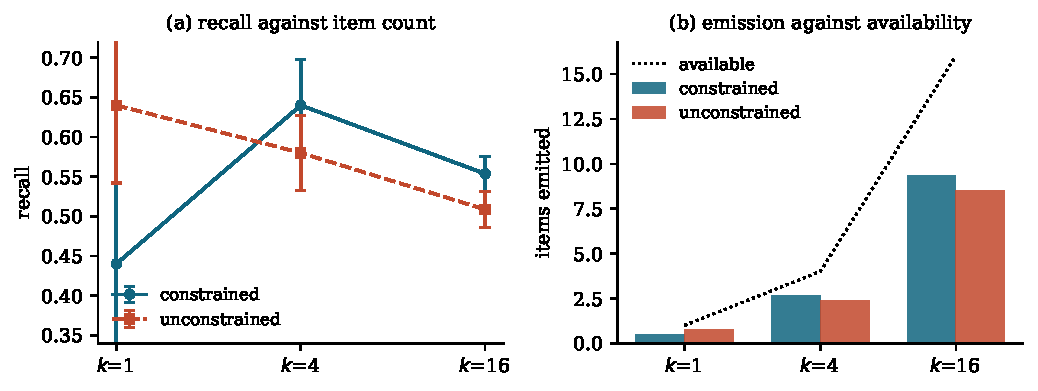
\includegraphics[width=\textwidth]{figures/cardinality.pdf}
\caption{(a) Recall against item count for both decoding regimes, 75 matched
documents per arm, error bars one standard error. The arms cross between $k=1$
and $k=4$. (b) Items emitted against items available. Both arms fall away from
availability as $k$ grows; the constrained arm slightly less.}
\label{fig:main}
\end{figure}

\begin{table}[h]
\centering
\small
\begin{tabular}{lrrrr}
\toprule
$k$ & constrained & unconstrained & paired difference & $p$ \\
\midrule
1 & 0.440 & 0.640 & $+0.200$ & 0.096 \\
4 & 0.640 & 0.580 & $-0.060$ & 0.185 \\
16 & 0.554 & 0.509 & $-0.045$ & 0.026 \\
\bottomrule
\end{tabular}
\caption{Recall by item count and decoding regime, paired on identical documents;
$p$ from a paired $t$-test on the per-document differences
(\code{score\_decoding.py}).}
\label{tab:main}
\end{table}

The pre-registered test rejects for neither arm. Unconstrained decoding drops
$0.131$ from $k \le 3$ to $k \ge 16$ with Spearman $-0.255$, $p = 0.027$: the
rank test clears $p < 0.05$ but the drop is below the 0.15 the rule requires.
Constrained decoding drops $-0.114$, meaning recall rises, with Spearman
$+0.041$, $p = 0.73$, satisfying neither condition. An earlier version of this
paper reported $0.214$ and $p = 0.011$ for the unconstrained arm and called it a
rejection; the difference is entirely the six parser failures described in
Section~4, which sat at $k = 4$ (two) and $k = 16$ (four).

The $k = 1$ comparison favours unconstrained decoding by 0.200 at $p = 0.096$.
Per-document recall at $k = 1$ is close to a Bernoulli draw, and the variance
arithmetic implies 106 documents are needed to detect a 0.15 difference at 80\%
power against the 25 run.

\paragraph{The interaction test.} The pre-registered test is applied to each arm
separately and never tests whether the slope differs between arms. That test was
added after the data were in and is reported as such
(\code{scripts/interaction\_test.py}). Regressing the paired difference,
unconstrained minus constrained, on $\log_2 k$ gives a slope of $-0.061$ per
doubling (s.e.\ 0.026, $p = 0.020$); Spearman of the paired difference against
$k$ is $-0.291$ ($p = 0.011$). At $k = 1$ the constrained arm returns an empty
list on 13 of 25 documents, against 8 of 25 unconstrained, and those 13 documents
carry the interaction: with them removed the slope is $+0.027$ ($p = 0.17$) and
Spearman is $-0.034$ ($p = 0.79$). Within the unconstrained arm alone, recall
from $k = 4$ to $k = 16$ falls from 0.580 to 0.509 with Spearman $-0.233$
($p = 0.10$); within the constrained arm the same comparison falls from 0.640 to
0.554 with Spearman $-0.237$ ($p = 0.10$). Above $k = 1$ the two arms decline
together. The between-arm difference in recall is therefore a property of the
one level the study's own power arithmetic and validity gate both flag as
unreliable, and it is not a finding.

\paragraph{Validity, the effect that has an artifact.} The share of responses
that are valid JSON as emitted, before any repair, is 25/25, 23/25 and 21/25 at
$k = 1, 4, 16$ without a grammar and 75/75 with one
(\code{json\_valid} in the scorer; \code{paper/json\_validity.txt} from
\code{scripts/json\_validity.py}, and the ``valid JSON'' column of
\code{project/reports/decoding\_result.txt}). The failures are not truncation
and not refusal: they are complete objects that break the format by quoting a
filing's own short form inside a string. That is the concrete thing a grammar
buys at high item counts in this study, and it is the thing a production system
without a repair step would have lost.

\paragraph{Emission counts.} At $k = 16$ the constrained arm emits 9.4 of 16
available items and the unconstrained arm 8.5, at precision 0.946 and 0.953
respectively. Both arms stop well short of the 16 available. The schema is a bare
\code{list[Link]} with no minimum length, so the grammar permits closing the
array after any element, including after none, and the constrained arm does stop
early and emits an empty list on 13 of 25 documents at $k = 1$. An earlier draft
attributed a larger emission gap to a partially filled array failing to parse;
that is false for this schema, and most of the gap was the parser defect. The
manipulation that would test a grammar-level stopping account, a
\code{minItems} bound or a required count field, was not run.

\paragraph{Cost.} Unconstrained decoding is not cheaper. It costs $1.1\times$ the
tokens at $k = 1$ and $0.7\times$ at $k = 16$: on this model it is both less
accurate at high $k$ and no less expensive.

\section{Scope conditions}

One model, dense, one family; nothing here separates architecture from decoding
regime. The reasoning-mode flag on this stack changes only which response field
the same tokens arrive in, verified by identical evaluation counts, so this work
says nothing about inference-time reasoning. The item bank is drawn from a single
domain and was screened with a different model (\code{qwen3:30b-a3b}) from the
one evaluated (\code{qwen3:14b}), so the bank is not guaranteed recoverable at
$k = 1$ by the evaluated extractor, which is one candidate explanation for the
failed gate. Absolute recall levels are not interpretable, both for that reason
and because the validity gate was not met. The between-arm recall contrast rests
on $k = 1$, the level that is underpowered by the study's own arithmetic, and the
pre-registered rule rejects for neither arm. Twenty-five documents per level and one model is a pilot
scale; the next run needs at least 100 documents per level and more than one
model family.

\section{Conclusion}

On the axis of how many items a model must emit, this pilot does not find that
the grammar costs recall, and it does not find that the grammar protects it.
Under the pre-registered rule neither decoding regime rejects the null. The
between-arm gap is real on the full sample and is carried by the $k = 1$ level,
where the constrained arm under-emits and the study's validity gate was not met;
above $k = 1$ the arms decline together. What the grammar demonstrably buys is
validity: without it, one response in five at $k = 16$ is not valid JSON as
emitted, and a scorer without a repair step reads those as zero recall, which is
how an earlier version of this paper came to report a rejection it did not have.

For practitioners the implication is narrower than the earlier title suggested:
on this model, free-form generation with post-hoc parsing, often proposed as an
escape from grammar masking~\citep{letmespeak}, costs no fewer tokens and
produces output that must be repaired before it can be scored, and whether it
costs recall is not settled at 25 documents per level. For evaluation, a single
$F_1$ over a benchmark whose $k$ distribution is unstated is not comparable across
benchmarks, because it averages over a mix nobody reported, and a tolerant parser
is part of the instrument and has to be tested like one.

\paragraph{Reproduction.} Code, pre-registration, the constructed evaluation set
and all 450 raw model responses are released at
\url{https://github.com/quantraunak/cardinality-eval}. The reported result
re-scores without a GPU.

\begin{thebibliography}{99}

\bibitem[Beurer-Kellner et~al.(2024)]{domino}
L.~Beurer-Kellner, M.~Fischer, and M.~Vechev.
\newblock Guiding LLMs the right way: Fast, non-invasive constrained generation.
\newblock In \emph{ICML}, 2024. arXiv:2403.06988.

\bibitem[Ferguson et~al.(2026)]{extractbench}
N.~Ferguson, J.~Pennington, N.~Beghian, A.~Mohan, D.~Kiela, S.~Agrawal, and
  T.~H. Nguyen.
\newblock ExtractBench: A benchmark and evaluation methodology for complex
  structured extraction.
\newblock arXiv:2602.12247, 2026.

\bibitem[Geng et~al.(2023)]{gcd2023}
S.~Geng, M.~Josifoski, M.~Peyrard, and R.~West.
\newblock Grammar-constrained decoding for structured NLP tasks without
  finetuning.
\newblock In \emph{EMNLP}, 2023. arXiv:2305.13971.

\bibitem[Geng et~al.(2025)]{jsonschemabench}
S.~Geng et~al.
\newblock Generating structured outputs from language models: Benchmark and
  studies.
\newblock arXiv:2501.10868, 2025.

\bibitem[Hong et~al.(2025)]{contextrot}
K.~Hong, A.~Troynikov, and J.~Huber.
\newblock Context rot: How increasing input tokens impacts LLM performance.
\newblock Chroma technical report,
  \url{https://www.trychroma.com/research/context-rot}, 2025.

\bibitem[Hsieh et~al.(2024)]{ruler}
C.-P. Hsieh et~al.
\newblock RULER: What's the real context size of your long-context language
  models?
\newblock arXiv:2404.06654, 2024.

\bibitem[LangChain(2024)]{multineedle}
LangChain.
\newblock Multi needle in a haystack.
\newblock \url{https://www.langchain.com/blog/multi-needle-in-a-haystack}, 2024.

\bibitem[Levy et~al.(2024)]{sametask}
M.~Levy, A.~Jacoby, and Y.~Goldberg.
\newblock Same task, more tokens: The impact of input length on the reasoning
  performance of large language models.
\newblock In \emph{ACL}, 2024. arXiv:2402.14848.

\bibitem[Liu et~al.(2024)]{lostinmiddle}
N.~F. Liu, K.~Lin, J.~Hewitt, A.~Paranjape, M.~Bevilacqua, F.~Petroni, and
  P.~Liang.
\newblock Lost in the middle: How language models use long contexts.
\newblock \emph{Transactions of the Association for Computational Linguistics},
  12:157--173, 2024.

\bibitem[Modarressi et~al.(2025)]{nolima}
A.~Modarressi, H.~Deilamsalehy, F.~Dernoncourt, T.~Bui, R.~A. Rossi, S.~Yoon,
  and H.~Sch\"utze.
\newblock NoLiMa: Long-context evaluation beyond literal matching.
\newblock arXiv:2502.05167, 2025.

\bibitem[Singhania et~al.(2024)]{recallthemall}
S.~Singhania, S.~Razniewski, and G.~Weikum.
\newblock Recall them all: Retrieval-augmented language models for long object
  list extraction from long documents.
\newblock arXiv:2405.02732, 2024.

\bibitem[Song et~al.(2025)]{countingstars}
M.~Song, M.~Zheng, and X.~Luo.
\newblock Counting-Stars: A multi-evidence, position-aware, and scalable
  benchmark for evaluating long-context large language models.
\newblock In \emph{COLING}, 2025. arXiv:2403.11802.

\bibitem[Wu et~al.(2024)]{longgenbench}
Y.~Wu, M.~Hee, Z.~Hu, and R.~K.-W. Lee.
\newblock LongGenBench: Benchmarking long-form generation in long context LLMs.
\newblock arXiv:2409.02076, 2024.

\bibitem[Tam et~al.(2024)]{letmespeak}
Z.~R. Tam, C.-K. Wu, Y.-L. Tsai, C.-Y. Lin, H.-y. Lee, and Y.-N. Chen.
\newblock Let me speak freely? A study on the impact of format restrictions on
  performance of large language models.
\newblock In \emph{EMNLP Industry Track}, 2024. arXiv:2408.02442.

\bibitem[Willard and Louf(2023)]{outlines}
B.~T. Willard and R.~Louf.
\newblock Efficient guided generation for large language models.
\newblock arXiv:2307.09702, 2023.

\bibitem[.txt(2024)]{saywhatyoumean}
.txt Engineering.
\newblock Say what you mean: A response to ``Let Me Speak Freely''.
\newblock \url{https://blog.dottxt.ai/say-what-you-mean.html}, 2024.

\end{thebibliography}

\end{document}
